\subsection{Branches and Tags}

Technically Subversion does not introduce separate concepts for branches and tags. Both branches and tags are versioned directories under repository root. As result Translator performs theirs translation in similar way. There are differences at Git level only:
\begin{enumerate}
	\compactlist
	\item Addition.
	\begin{itemize}
		\item Creation of /branches/\emph{B} directory leads to creation of a new branch reference \emph{B}.
		\item Creation of /tags/\emph{T} directory leads to addition of corresponding Tag Object with name \emph{T}.
	\end{itemize}
	\item Modification.
	\begin{itemize}
		\item Change at /branches/\emph{B} directory leads to updating of corresponding branch reference \emph{B}.
		\item Change at /tags/\emph{T} directory leads to the removal of obsolete Tag Object with name \emph{T} and creation of new Tag Object with the same name for corresponding Commit Object.
	\end{itemize}
	\item Deletion.
	\begin{itemize}
		\item Removal of /branches/\emph{B} directory leads to removal of corresponding reference \emph{B} at Git repository, when
		\item Removal of /tags/\emph{T} directory leads to removal of corresponding Tag Object with name \emph{T}.
	\end{itemize}
\end{enumerate}

The same rules could be treated in opposite direction --- every change of Git branch or tag leads to corresponding change of Subversion branch or tag.

This and further chapters consider scenarios with branches only. Every scenario could be applied to tags with the rules above taken into account.

\subsubsection{Creation}

There is a couple of ways to create branch in Subversion by keeping history of another branch:

\begin{enumerate}
\compactlist
\renewcommand{\figurename}{Diagram}
\item Branch creation by copying, diagram \ref{branch_creation_svn_to_git}.
\begin{figure}[!h]
\centering
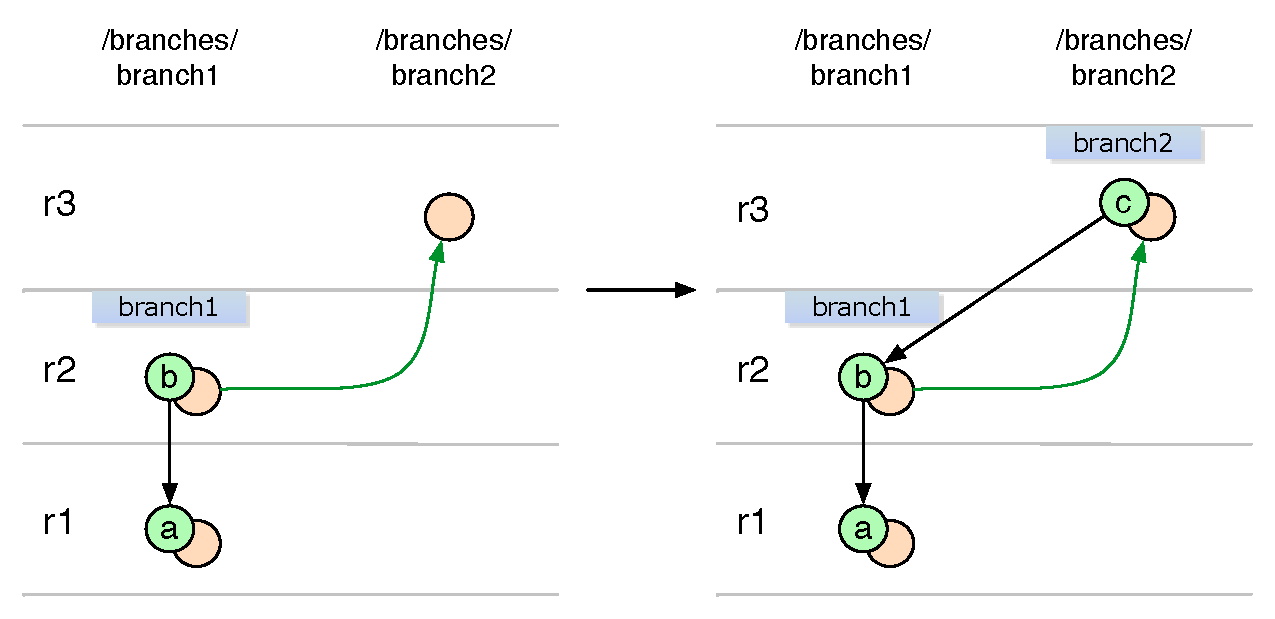
\includegraphics[width=\linewidth]{img/diagrams/branch_creation_svn_to_git.pdf}
\caption{Subversion branch copying being translated to Git branch creation.}
\label{branch_creation_svn_to_git}
\end{figure}

\item Branch creation with merge history, diagram \ref{branch_creation_from_mergeinfo_svn_to_git}.
\begin{figure}[!h]
\centering
\renewcommand{\figurename}{Diagram}
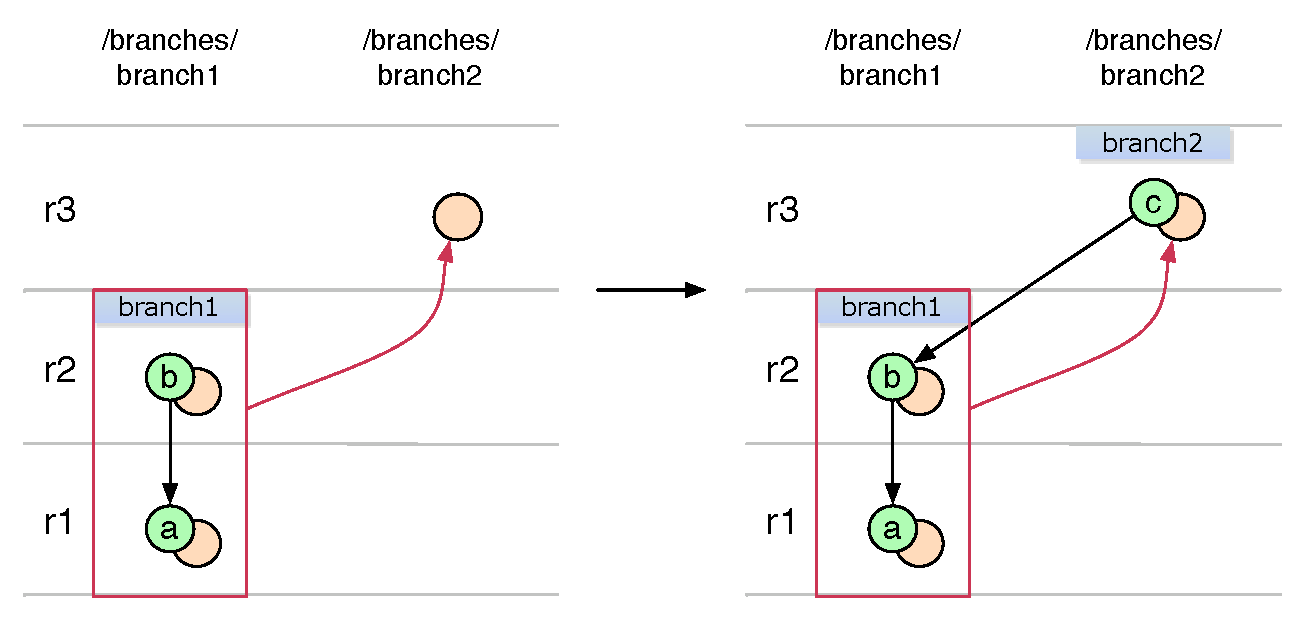
\includegraphics[width=\linewidth]{img/diagrams/branch_creation_from_mergeinfo_svn_to_git.pdf}
\caption{Subversion branch addition being translated to Git branch creation.}
\label{branch_creation_from_mergeinfo_svn_to_git}
\end{figure}
\end{enumerate}

In opposite direction translation behaves as depicted at diagram \ref{branch_creation_git_to_svn}.
\begin{figure}[!h]
\centering
\renewcommand{\figurename}{Diagram}
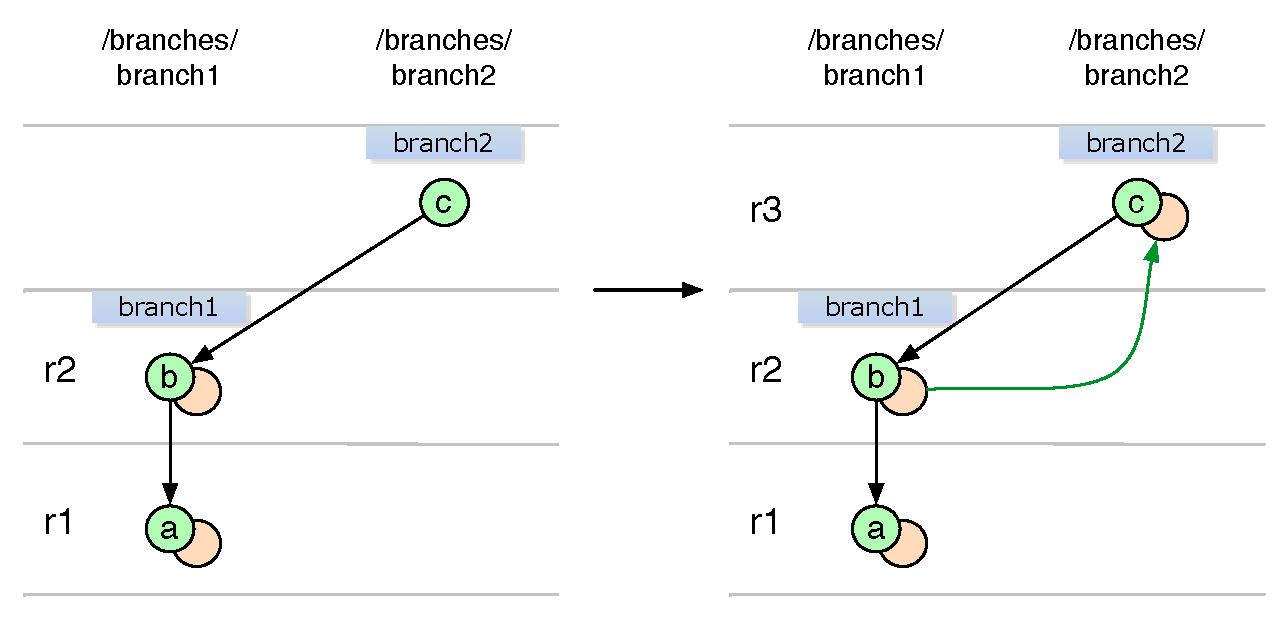
\includegraphics[width=\linewidth]{img/diagrams/branch_creation_git_to_svn.pdf}
\caption{Subversion branch addition being translated to Git branch creation.}
\label{branch_creation_git_to_svn}
\end{figure}

Branches also could be created with no history. This kind of Subversion to Git translation depicted at diagram \ref{branch_creation_no_history_svn_to_git} and corresponding Git to Subversion translation depicted at diagram \ref{branch_creation_no_history_git_to_svn}.

\begin{figure}[!h]
\centering
\renewcommand{\figurename}{Diagram}
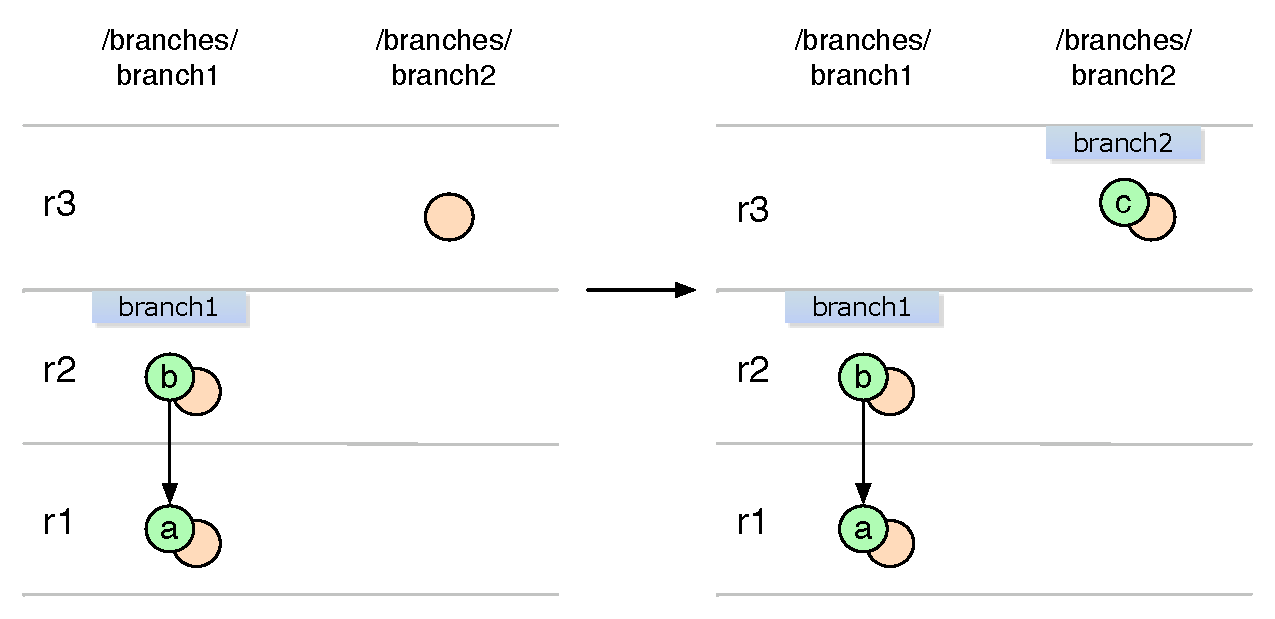
\includegraphics[width=\linewidth]{img/diagrams/branch_creation_no_history_svn_to_git.pdf}
\caption{Subversion branch addition being translated to Git branch creation.}
\label{branch_creation_no_history_svn_to_git}
\end{figure}

\begin{figure}[!h]
\centering
\renewcommand{\figurename}{Diagram}
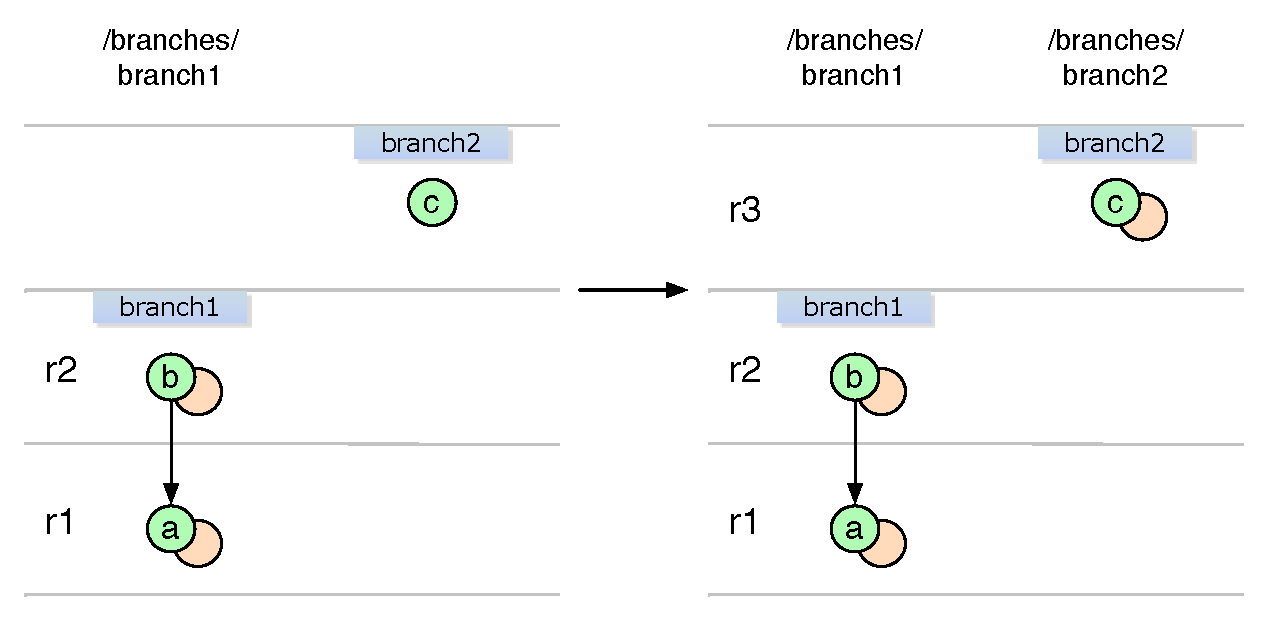
\includegraphics[width=\linewidth]{img/diagrams/branch_creation_no_history_git_to_svn.pdf}
\caption{Subversion branch addition being translated to Git branch creation.}
\label{branch_creation_no_history_git_to_svn}
\end{figure}

\subsubsection{Modification}

\subsubsection{Deletion}

\subsubsection{Replacement}
